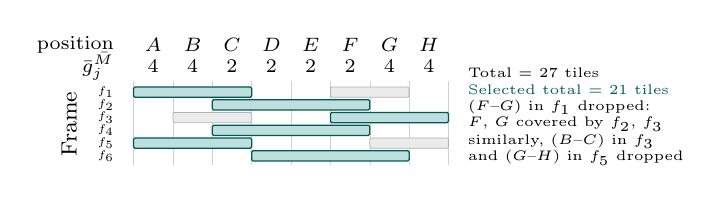
\begin{tikzpicture}[x=0.5cm,y=0.54cm]
  \tikzstyle{labelstyle}=[font=\footnotesize]
  \tikzstyle{guidestyle}=[line width=0.2pt, draw=black!18]
  \tikzstyle{dropstyle}=[draw=black!30, fill=black!8, rounded corners=0.5pt, line width=0.3pt]
  \tikzstyle{keepstyle}=[draw=teal!70!black, fill=teal!25, rounded corners=0.5pt, line width=0.45pt]
  \tikzstyle{countstyle}=[font=\footnotesize, text=teal!70!black]

  \foreach \x/\name/\c in {0/A/4,1/B/4,2/C/2,3/D/2,4/E/2,5/F/2,6/G/4,7/H/4} {
    \node[labelstyle, font=\scriptsize] at (\x+0.5,1.05) {$\name$};
    \node[labelstyle, font=\scriptsize] at (\x+0.5,0.55) {$\c$};
    \draw[guidestyle] (\x,0.2) -- (\x,-1.77);
    \draw[guidestyle] (\x+1,0.2) -- (\x+1,-1.77);
  }
  \node[labelstyle, font=\scriptsize, anchor=east] at (-0.25,1.05) {position};
  \node[labelstyle, font=\scriptsize, anchor=east] at (-0.25,0.55) {$\bar{g}_j^{\bar{M}}$};

  \node[labelstyle, rotate=90, anchor=south] at (-1.2,-0.8) {Frame};
  \foreach \y/\t in {-0.05/f_1,-0.35/f_2,-0.65/f_3,-0.95/f_4,-1.25/f_5,-1.55/f_6} {
    \node[labelstyle, font=\tiny, anchor=east] at (-0.25,\y) {\scalebox{0.8}{$\t$}};
  }

  % t1: keep (A-B-C), drop (F-G) — PARTIAL
  \draw[keepstyle] (0,-0.17) rectangle (3,0.07);
  \draw[dropstyle] (5,-0.17) rectangle (7,0.07);

  % t2: keep (C-D-E-F)
  \draw[keepstyle] (2,-0.47) rectangle (6,-0.23);

  % t3: drop (B-C), keep (F-G-H) — PARTIAL
  \draw[dropstyle] (1,-0.77) rectangle (3,-0.53);
  \draw[keepstyle] (5,-0.77) rectangle (8,-0.53);

  % t4: keep (C-D-E-F)
  \draw[keepstyle] (2,-1.07) rectangle (6,-0.83);

  % t5: keep (A-B-C), drop (G-H) — PARTIAL
  \draw[keepstyle] (0,-1.37) rectangle (3,-1.13);
  \draw[dropstyle] (6,-1.37) rectangle (8,-1.13);

  % t6: keep (D-E-F-G)
  \draw[keepstyle] (3,-1.67) rectangle (7,-1.43);

  \node[labelstyle, font=\tiny, anchor=west] at (8.25,0.4) {Total = 27 tiles};
  \node[countstyle, font=\tiny, anchor=west] at (8.25,0.0) {Selected total = 21 tiles};
  \node[labelstyle, font=\tiny, anchor=west, align=left] at (8.25,-0.6) {$(F$--$G)$ in $f_1$ dropped:\\
  $F$, $G$ covered by $f_2$, $f_3$};
  \node[labelstyle, font=\tiny, anchor=west, align=left] at (8.25,-1.4) {similarly, $(B$--$C)$ in $f_3$\\
  and $(G$--$H)$ in $f_5$ dropped};
\end{tikzpicture}
